% easychair.tex,v 3.0 2011/10/24
%
% Select appropriate paper format in your document class as
% instructed by your conference organizers. Only withtimes
% and notimes can be used in proceedings created by EasyChair
%
% The available formats are 'letterpaper' and 'a4paper' with
% the former being the default if omitted as in the example
% below.
%
%\documentclass{easychair}
\documentclass[]{easychair}
%\documentclass[verbose]{easychair}
%\documentclass[notimes]{easychair}
%\documentclass[withtimes]{easychair}
%\documentclass[a4paper]{easychair}
%\documentclass[letterpaper]{easychair}
%\documentclass[notimes,custompaper,lmargin=1cm,rmargin=2cm,tmargin=.5cm,bmargin=1.5cm]{easychair}
%\documentclass[notimes,custompaper,lmargin=1cm,rmargin=2cm,tmargin=.5cm,bmargin=1.5cm]{easychair}

% This provides the \BibTeX macro
\usepackage{doc}
\usepackage{makeidx}

% In order to save space or manage large tables or figures in a
% landcape-like text, you can use the rotating and pdflscape
% packages. Uncomment the desired from the below.
%
% \usepackage{rotating}
% \usepackage{pdflscape}

% If you plan on including some algorithm specification, we recommend
% the below package. Read more details on the custom options of the
% package documentation.
%
% \usepackage{algorithm2e}

% Some of our commands for this guide.
%
\usepackage{xspace}
\usepackage{amssymb}
\usepackage{color}
\newcommand{\comment}[4]{\par\noindent\hspace*{-0.5cm}{\parbox{\columnwidth}{\textbf{\color{#1}//#2[#3]:#4}}}\par}

\newcommand{\easychair}{\textsf{easychair}}
\newcommand{\miktex}{MiK{\TeX}}
\newcommand{\texniccenter}{{\TeX}nicCenter}
\newcommand{\makefile}{\texttt{Makefile}}
\newcommand{\latexeditor}{LEd}
\newcommand{\ex}[1]{\emph{ex.}\xspace\emph{#1}}
\newcommand{\ie}[0]{\emph{c-à-d.}\xspace}
\newcommand{\mi}[1]{\comment{blue}{}{#1}{MI}}
\newcommand{\ch}[1]{\comment{green}{}{#1}{CH}}
\newcommand{\si}[1]{\comment{red}{}{#1}{SI}}
\newcommand{\FM}[0]{\textsc{fm}\xspace}
\newcommand{\Y}[0]{\textsc{YourCast}\xspace}
\newcommand{\LP}[0]{{ligne de produits}\xspace}
\newcommand{\LPS}[0]{{lignes de produits}\xspace}
\newcommand{\IR}[0]{interFMRelation}%\xspace}
\newcommand{\source}[0]{\textsc{source}\xspace}
\newcommand{\policy}[0]{\textsc{policy}\xspace}

%\makeindex

%% Document
%%
\begin{document}

%% Front Matter
%%
% Regular title as in the article class.
%
\title{Vers la composition de workflows pour le filtrage sémantique de nouvelles}

% \titlerunning{} has to be set to either the main title or its shorter
% version for the running heads. Use {\sf} for highlighting your system
% name, application, or a tool.
%
\titlerunning{Workflows de filtrage sémantique de nouvelles}

% For only the editors. Authors, please keep this commented out
% \volumeinfo
% 	{G. Sutcliffe, A. Voronkov}         % editors
% 	{2}                                 % number of editors
%	{{\easychair} 3.0 Beta 5, March 2011}      % event
%	{2}                                 % volume
%	{1}                                 % issue
%	{1}                                 % starting page number
%\indexededitor{Sutcliffe, Geoff}
%\indexededitor{Voronkov, Andrei}

%\headfootstyle
%	{}
%	{\sf}
%	{\footnotesize\sf}
%	{\small}

\volumeinfoECPS
	{CIEL Proceedings}
	{ECPS vol. 7999}

% Authors are joined by \and and their affiliations are on the
% subsequent lines separated by \\ just like the article class
% allows.
%
\author{
    Christophe Desclaux\\
    \affiliation{Université Nice Sophia Antipolis}\\
    \affiliation{\url{christophe@zouig.org}}\\
\and
    Simon Urli\\
    \affiliation{I3S, CNRS}\\
    \affiliation{Université Nice Sophia Antipolis}\\
    \affiliation{\url{urli@i3s.unice.fr}}\\
\and
    Mireille Blay-Fornarino\\
    \affiliation{I3S, CNRS}\\
    \affiliation{Université Nice Sophia Antipolis}\\
    \affiliation{\url{blay@polytech.unice.fr}}\\
\and
    Catherine Faron Zucker\\
    \affiliation{I3S, CNRS}\\
    \affiliation{Université Nice Sophia Antipolis}\\
    \affiliation{\url{faron@polytech.unice.fr}}\\
}

% \authorrunning{} has to be set for the shorter version of the authors' names;
% otherwise a warning will be rendered in the running heads.
%
\authorrunning{Desclaux, Urli, Blay-Fornarino and Faron Zucker}
\indexedauthor{Christophe, Desclaux}
\indexedauthor{Simon, Urli}
\indexedauthor{Mireille, Blay-Fornarino}
\indexedauthor{Catherine, Faron Zucker}

%%%%%%%%%%%%%%%%%%%%%%%%%%%%%%%%%%%%%%%%%%%%%%%%%%%
\maketitle
%%%%%%%%%%%%%%%%%%%%%%%%%%%%%%%%%%%%%%%%%%%%%%%%%%%
%------------------------------------------------------------------------------
% Abstract
%
\begin{abstract}
\ch{je ne sais pas comment écrire abstract en francais avec LaTex}
Le web se révèle aujourd'hui un merveilleux support de diffusion d'informations. Cependant, tandis que les sources se multiplient (flux rss, services web, ..), la quantité d'informations croît et il est difficile de les filtrer en fonction des centres d'intérêts des utilisateurs. Actuellement de nombreux outils qui exploitent les ontologies ou les thésaurus sont mis au point. Ils permettent d'annoter les informations, d'en déduire des critères et d'ensuite obtenir uniquement les informations pertinentes. La composition de ces outils constitue des workflows qui devraient encore s'enrichir grâce à l'apparition de nouvelles ontologies ciblées sur différents domaines et outils de lecture.  Cependant la construction de telles chaînes logicielles n'est pas à la portée de tous. \\
Dans cet article nous montrons comment de tels workflows ont été construits et présentons nos perspectives en matière de construction automatique de ces workflows en fonction des besoins utilisateur. Ce travail s'appuie sur le projet ANR EMergence Yourcast qui vise à automatiser la diffusion des informations sur de grands écrans, et pour lequel la pertinence des informations diffusées est donc particulièrement pertinent. 
\end{abstract}

\begin{abstract}
Internet is becoming today a wonderful medium for disseminating information. While the sources are multiplying (RSS, Web Services, ...), the amount of information is growing and it becomes difficult to filter them according to user interests. Many tools are currently developed that exploits ontologies or thesauri to annotate informations. They enable to query these annotations according to criteria to retrieve only the relevant information. The composition of these tools constitute workflows that should be enriched by the emergence of new ontologies modeling different domains and text analysis tools. However the composition of this tools-chain is not for everyone.\\
In this paper we show how these workflows are built and present our approach for automatically building workflows based on user needs. This work is supported by the ANR Emergence Yourcast project dedicated to automate the dissemination of information on large screens, and for which the relevance of the information published is particularly relevant.
\end{abstract}

\section{Mots clé}
Semantic Web, Product Line, Workflow
\ch{ je ne sais pas comment formaliser les mots clé avec ce template}
%------------------------------------------------------------------------------

\section{Introduction}
\label{sect:introduction}
%Mi{N'aime pas le titre}

Le web se révèle aujourd'hui un merveilleux support de diffusion d'informations. Tandis que les sources se multiplient (flux rss, services web, ..), la quantité des informations croît et il devient difficile de les filtrer en fonction des centres d'intérêts des utilisateurs \cite{Bouzeghoub2005}. Des outils qui exploitent des ontologies ou des thésaurus ont été mis au point qui permettent d'annoter les informations, d'en déduire des critères et d'ensuite obtenir uniquement les informations pertinentes en formulant des requêtes sémantiques sur les annotations. 
%\mi{enrichir ce qui précède avec des références en essayant si possible de faire ressentir les éléments de l'architecture.}

Il devient aujourd'hui possible de construire à la fois des workflows mettant en jeu ces différents outils pour annoter les flux d'informations pour sélectionner les informations. 
Cependant la construction de ces workflows reste technique malgré les nouveaux supports logiciels tels que les mashup \cite{Floyd2007} \cite{Milanovic2004}. En effet elle se base sur de nombreux critères qui doivent être pris en compte pour assembler les services et le fait que ces services soient hétéroclites ne permet pas une génération aisée des applications. De plus de nouvelles ontologies, sources, systèmes d'annotations apparaissent régulièrement tandis que le web se démocratise \cite{Anderruthy2007} \cite{Bross2010}.
%\mi{et surtout bien le dire}
Dans ce contexte, nous abordons dans cet article la production automatique de ces workflows à partir d'un ensemble de caractéristiques proposées à l'utilisateur. 

Nous présentons en section \ref{sect:exemple} le contexte de notre travail que s'inscrit dans le cadre du projet ANR EMergence Yourcast qui vise à automatiser la diffusion des informations sur de grands écrans. Nous montrons au travers d'un cas d'étude les différents choix qui se posent à l'utilisateur et décrivons dans la section \ref{sect:miseEnOuvre} les workflows  mis en place pour répondre à ce cas particulier. Fort de cette expérience, nous proposons en section \ref{sect:perspectives} de produire de tels workflows en utilisant un développement dirigé par les modèles et les feature models. 


%------------------------------------------------------------------------------

\section{Contexte et besoins exprimés dans le projet YourCast}
\label{sect:exemple}
Dans le cadre du projet \Y, nous visons à diffuser sur de grands écrans des informations en provenance de différentes sources en particulier celles issues du web. Or de tels systèmes exigent une adhérence forte aux attentes des utilisateurs et l'adéquation des informations avec les centres d'intérêts des personnes est essentielle à l'acceptation de tels systèmes. 

%\paragraph*{Des sources hétérogènes} <= Supprimé par Catherine
\ch{Je prefere qu'on garde les sous titre ici cependant Catherine souhaite les enlever : à Mireille de trancher (ca évite selon moi l'effet bloc de texte chiant à lire)}

Il existe aujourd'hui de nombreuses sources d'information disponibles grâce à l'utilisation de flux RSS. Le choix des sources peut être simplement lié au travail ou à l'emplacement géographique de l'écran d'information.
Dans notre cas, nous avons choisi d'agréger le plus de sources d'informations possible pour couvrir tous les champs d'application des écrans d'accueil. 
Nous faisons donc appel dans notre application à une vingtaine de flux RSS sur de vastes sujets. Ceux-ci sont essentiellement des flux ayant déjà subi une étape de filtrage qui a permis de les classer selon leurs thématiques générales (technologies, international, médical, ...).

%\paragraph*{Sélection des informations}
Beaucoup de sources d'informations sont agrégeables. Des critères de sélection sont alors pré-établis par les fournisseurs de contenus.  Par exemple sur le site de news de Google\footnote{\url{http://news.google.fr}} l'internaute peut accéder à des nouvelles liées à l'économie ou bien des news locales. Cependant il ne peut pas récupérer les nouvelles économiques liées par exemple à la ville de Marseille ou plus largement à la région PACA. Dans notre exploitation des flux RSS nous souhaitons fournir un filtrage multi-critères permettant un tri fin des nouvelles. 

%\paragraph*{Des critères utilisateurs}
Pour capturer ces critères il existe actuellement différents systèmes tels que le service \textsl{Google Reader}\footnote{\url{http://www.google.fr/reader/}} ou bien celui \textsl{rssLounge}\footnote{\url{http://rsslounge.aditu.de}}. Cependant ceux-ci ne proposent pas de regroupement des flux ni de filtrage multi-critère de ceux-ci.
Or le besoin exprimé dans le projet \Y est celui d'un système intuitif qui permette de capturer simplement les exigences utilisateur. Nous avons pour cela développé un système d'aide au choix qui après captation en langage naturel des besoins les retranscrit sous forme d'entités nommées qui sont typées par notre système en fonction des éléments que nous avons déjà pu instancier dans la base de connaissances.

%\paragraph*{Des processus d'annotation diversifiés}
Le système est basé sur une annotation des informations la plus vaste possible. En effet le système doit pouvoir annoter des informations provenant de domaines totalement différents.
Nous avons choisis d'utiliser des annotions basées sur la récupération d'entités nommées présentes sur un grand nombre de bases de données RDF.
Nous utilisons alors des systèmes d'extraction d'information et d'annotation sémantique qui permettent d'ajouter des liaisons vers les entités nommées spécifiques.


%------------------------------------------------------------------------------

\section{Annotation et filtrage sémantiques de flux RSS}
\label{sect:miseEnOuvre}
Pour répondre aux besoins exprimés dans le cadre du projet \Y nous avons mis au point deux workflows, dont la figure 1 présente  l'architecture générale: un workflow d'enrichissement sémantique des nouvelles (en bleu) et un workflow de filtrage sémantique des nouvelles. La scicion en deux workflows est essentielle car elle permet de faire travailler nos workflows de manière asynchrone.
 \ch{je présente peut etre la notion de workflow asynchrone de manière maladroite?}

\begin{figure}[htb!]
	\begin{centering}
	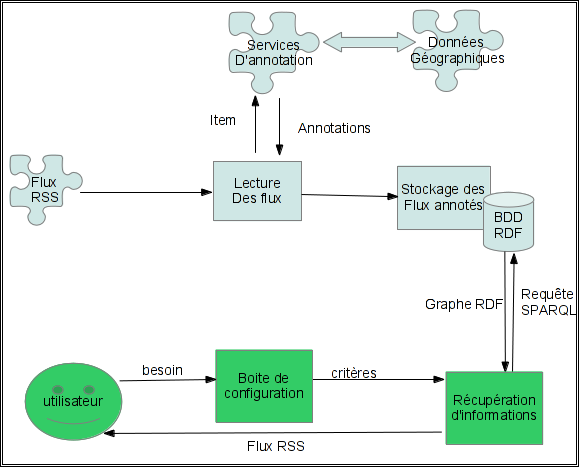
\includegraphics[width=0.9\textwidth]{diagramme-Archi.png}
	\caption{Workflows d'annotation et de filtrage sémantique de nouvelles}
	\label{fig:mmFM}
	\end{centering}
\end{figure}

\subsection{Workflow d'enrichissement sémantique des nouvelles}

\subsubsection{Lecture de flux RSS}
Le workflow se base sur la récupération de flux RSS qui sont choisis par l'utilisateur et dont nous connaissons le thème et la langue, chaque flux RSS contient un lot de nouvelles les plus récentes publiées chez le fournisseur du flux. Le flux peut être mis à jour et doit être interrogé périodiquement pour récupérer les dernières nouvelles publiées.

\subsubsection{Annotation sémantique de nouvelles}
Pour chaque nouvelle, nous utilisons des services d'annotation pour récupérer les entités nommées intéressantes la concernant: 
\begin{itemize}
	\item \textbf{OpenCalais}\footnote{http://www.opencalais.com} permet d'identifier dans le texte les entités correspondant à des lieux français ainsi que des noms de personnalités en langue anglaise. gràce à l'API Java fourni par le projet OpenCalais, nous avons implémenté le code permettant de récupérer les annotations textuelles concernant le texte à annoter;
  \item \textbf{WikiMeta}\footnote{http://www.wikimeta.com} fonctionne sur le même principe qu'OpenCalais. Cependant le projet ne proposait pas au moment de nos recherche d'API permettant d'effectuer des requêtes et nous avons alors du implémenter l'API Java se connectant à leurs service web. Elle permet de récupérer directement des entités nommées pointant vers la base de connaissances DBpedia; il peut donc être utilisé seul en tant que service d'annotation principal.
\end{itemize}

Nous faisons appel à des services de généralisation qui travaillent en aval des services d'annotation pour ajouter des notions à une annotation :
\begin{itemize}
	\item \textbf{DBpedia}\footnote{http://dbpedia.org} travaille sur les données provenant du service d'annotation WikiMeta et permet de les enrichir sémantiquement à l'aide de liens vers d'autres ressources liées à l'élément.
  \item \textbf{INSEE geo} \footnote{\url{http://rdf.insee.fr/geo/}} La base de données RDF de l'INSEE permet de récupérer les ensembles géographiques liés à une entité nommée géographique. Ce service d'annotation géographique s'utilise donc uniquement en aval d'un service d'annotation classique qui récupère des informations géographiques. Il renvoie des URI vers les entités géographiques liées à la nouvelle étudiée. Nous utilisons pour cela une requête SPARQL telle que celle ci-dessous qui permet de retrouver le nom et le type des subdivisions de la ville de Nice :
\end{itemize}

\begin{verbatim}
    PREFIX geo: <http://rdf.insee.fr/geo/>
    SELECT DISTINCT ?nom ?type WHERE {
	     ?entite geo:nom ?nom
	     ?entite rdf:type ?type
	     ?ville geo:nom ?nomVille
         ?entite geo:subdivision* ?ville
         FILTER(regex(str(?nomVille), 'Nice', 'i'))
    }
\end{verbatim}

\ch{nous n'avons pas présenté la partie mémorisation, est-ce grave?}
%\subsubsection{Mémorisation}
%\mi{je ne sens pas cette partie.. à voir}
%Nous stockons le contenu des flux RSS et les annotations dans une base de données RDF grâce à l'utilisation de l'application 4Store. 4store est un serveur de triplets RDF fournissant un accès aux données en lecture et écriture. Il nous permet de créer un EndPoint en ligne rapide et puissant. De plus, cela permet une réutilisation de notre travail d'annotations dans d'autres projets aillant besoin d'accéder à des flux annotés. Enfin cette technologie va permettre une excellente connection entre le workflow d'enrichissement et celui de filtrage car de nombreuses APIs existent pour attaquer la base de données dans différents langages.

\subsection{Workflow de filtrage des nouvelles}
Le workflow de filtrage permet de créer des critères utilisateurs afin de récupérer les données intéressantes sur la base des annotations. Notre workflow va dans un premier temps transformer les besoins utilisateurs en critères sous forme d'une liste de couples (TypeElement,entiteDescriptive). Ces couples sont ensuite envoyés à l'élément de connection à la base de données qui effectue une requête SPARQL multicritères sur la base de donnée RDF pour récupérer les nouvelles à fournir à l'utilisateur. Enfin le système génère un flux RSS personnalisé pour répondre aux besoins utilisateur et le fourni au client. Ce flux RSS va pouvoir être mémorisé par le client pour récupérer en temps réel les nouvelles informations.
%on choisi de ne pas détailler ce workflow

%Cath: il faudrait détailler davantage ce workflow, quitte à réduire la partie suivante
%Chris: vous etes sur? on pense qu'elle n'apporte pas enormement à notre reflection (on verra demain)
%------------------------------------------------------------------------------

\section{Vers la construction automatique de workflows }
\label{sect:perspectives}
Notre objectif à terme est de construire une ligne de produits qui capturerait les différentes sources et services disponibles, les qualifierait et permettrait à un utilisateur final de construire ses propres workflows d'annotation en le guidant dans sa sélection de différents services.

%\subsection{Objectifs} <= supprimé par Catherine
%chris: ok pour la suppression du titre
Du point de vue de l'utilisateur final, l'utilisation d'une construction de workflows pourrait lui permettre, à partir d'un flux sélectionné, d'affiner la sélection des services d'annotations qu'il souhaite utiliser afin d'obtenir l'information la plus complète pour son utilisation.

A l'heure actuelle le workflow d'annotation interroge tous les services d'annotations disponibles, sans distinction de catégories, ce qui génère de nombreux appels de services dont la plupart sont inutiles. L'utilisation d'une construction automatique à partir des choix de l'utilisateur permettrait de restreindre les appels aux seuls services pertinents et donc d'accélérer les temps de traitements en réduisant la charge des services. 

\subsection{Lignes de produits de services}
Les choix que va faire l'utilisateur vont avoir un impact sur trois concepts inhérents au workflow d'annotations : les \textit{Flux d'information}, les \textit{Services d'Annotation} et les \textit{Services de Généralisation}. Chacun de ces concepts peut être vu comme une ligne de produits (services) indépendante, à partir de laquelle l'utilisateur choisira le service qui lui convient. Nous représentons ces lignes de produits par des modèles d'aspects ou \textsl{feature models} (FM).

La figure 2 montre ainsi l'aspect \textit{Service d'Annotation} : les produits finaux correspondent aux feuilles de l'aspect \textit{Produit}, les thèmes aux feuilles de l'aspect \textit{Thème} et les langues à celles de l'aspect \textit{Langue}. La sélection d'un aspect de langue ou de thème influe directement sur le choix d'un service final par le jeu des contraintes internes au FM. 

%Cath : changer Product en Produit dans la figure

%Cath La qualité de la figure ne convient pas: elle est très floue à l'impression

\begin{figure}[htb!]
	\begin{centering}
	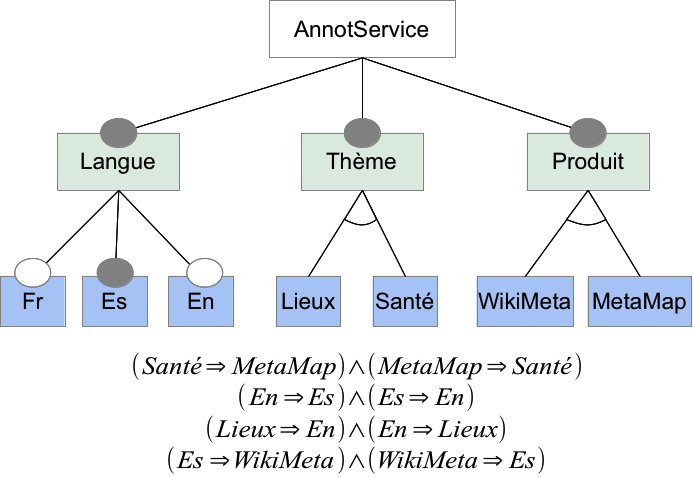
\includegraphics[scale=0.7]{FM.png}
	\caption{Workflow de traitements....}
	\label{fig:mmFM}
	\end{centering}
\end{figure}
%\si{à voir si on garde en dessous...}
%Chacun des FM des différents concepts est une construction réalisée à partir d'une approche bottom-up. Nous partons des produits existants, en les exprimant sous forme de FM individuels, puis nous effectuons la fusion de ces FM afin d'obtenir une SPL modélisant les différents produits disponibles ainsi que leur variabilité \cite{Acher2011}.

\subsection{Modèle de mise en relation des LPL}
Notre but est de fournir un outil permettant à un utilisateur final de sélectionner des services cohérents en fonction de ses choix. Cela implique que chaque choix que l'utilisateur fera dans un des FM doit avoir un impact sur les autres concepts du domaine. 
Nous exprimons donc des relations entre les différents concepts du domaine, relations qui s'expriment par le biais du \textit{Thème} et de la \textit{Langue}. En effet, les systèmes d'annotation sont spécialisés pour certains types d'informations, comme le service MetaMap \footnote{\url{http://metamap.nlm.nih.gov/}} et ne traitent que certaines langues. Une relation exprime à la fois qu'un produit (i.e. un service) sera lié à un autre, mais aussi que sélectionner un produit influera sur la sélection d'un autre.

Par exemple, un \textit{Flux} traitant de politique sera annoté par un ou plusieurs \textit{Services d'annotation} pouvant annoter ce type d'information : les produits seront donc liés. Cependant ce \textit{Flux} ne pourra pas être lié à un \textit{Service d'annotation} parlant d'un thème différent ou traitant une langue différente : la sélection du flux influe directement sur la sélection des \textit{Services d'annotation} à lier.

Pour cela nous définissons et appliquons des opérations de restrictions sur les relations entre les FMs, et ce en cascade. Pour reprendre notre exemple, la sélection d'un flux influe sur la sélection des annotations, en restreignant les services disponibles, ce qui aura également une influence sur les services de généralisation disponibles. 

%---------------------------------------------------------------
\section{Conclusion}
\label{sect:conclusion}
Dans cet article nous avons présenté le système d'annotation ZeOntologyNewsExtractor \footnote{\url{https://github.com/descl/ZONE}} dont nous présentons une preuve de concept sur \url{http://zone.zouig.org}. Nous avons explicité l'utilisation de l'ingénierie des connaissances pour enrichir sémantiquement des nouvelles. Puis nous avons présenté la nécessité de faire appel à l'ingénierie du logiciel et particulièrement la mise en place de workflows pour organiser les flux composant notre architecture. Enfin nous avons présenté une amélioration possible de notre approche utilisant la génération de lignes de produits logiciels. 
\ch{il faut une ouverture que je ne trouve pas}

%------------------------------------------------------------------------------
% Refs:
%

\label{sect:bib}
\bibliographystyle{plain}
%\bibliographystyle{alpha}
%\bibliographystyle{unsrt}
%\bibliographystyle{abbrv}
\bibliography{christophe}
\ch{il manque la biblio de simon sur les LDP}

%------------------------------------------------------------------------------
\appendix

%------------------------------------------------------------------------------
% Index
%\printindex

%------------------------------------------------------------------------------
\end{document}

% EOF
